\documentclass{article}
\usepackage{amsfonts,amssymb,amsmath,amsthm}

%% set-style letters
\def\AA{{\mathbb{A}}}
\def\BB{{\mathbb{B}}}
\def\CC{{\mathbb{C}}}
\def\DD{{\mathbb{D}}}
\def\EE{{\mathbb{E}}}
\def\FF{{\mathbb{F}}}
\def\GG{{\mathbb{G}}}
\def\HH{{\mathbb{H}}}
\def\II{{\mathbb{I}}}
\def\JJ{{\mathbb{J}}}
\def\KK{{\mathbb{K}}}
\def\LL{{\mathbb{L}}}
\def\MM{{\mathbb{M}}}
\def\NN{{\mathbb{N}}}
\def\OO{{\mathbb{O}}}
\def\PP{{\mathbb{P}}}
\def\QQ{{\mathbb{Q}}}
\def\RR{{\mathbb{R}}}
\def\SS{{\mathbb{S}}}
\def\TT{{\mathbb{T}}}
\def\UU{{\mathbb{U}}}
\def\VV{{\mathbb{V}}}
\def\WW{{\mathbb{W}}}
\def\XX{{\mathbb{X}}}
\def\YY{{\mathbb{Y}}}
\def\ZZ{{\mathbb{Z}}}

%% calligraphic letters
\def\cA{{\mathcal{A}}}
\def\cB{{\mathcal{B}}}
\def\cC{{\mathcal{C}}}
\def\cD{{\mathcal{D}}}
\def\cE{{\mathcal{E}}}
\def\cF{{\mathcal{F}}}
\def\cG{{\mathcal{G}}}
\def\cH{{\mathcal{H}}}
\def\cI{{\mathcal{I}}}
\def\cJ{{\mathcal{J}}}
\def\cK{{\mathcal{K}}}
\def\cL{{\mathcal{L}}}
\def\cM{{\mathcal{M}}}
\def\cN{{\mathcal{N}}}
\def\cO{{\mathcal{O}}}
\def\cP{{\mathcal{P}}}
\def\cQ{{\mathcal{Q}}}
\def\cR{{\mathcal{R}}}
\def\cS{{\mathcal{S}}}
\def\cT{{\mathcal{T}}}
\def\cU{{\mathcal{U}}}
\def\cV{{\mathcal{V}}}
\def\cW{{\mathcal{W}}}
\def\cX{{\mathcal{X}}}
\def\cY{{\mathcal{Y}}}
\def\cZ{{\mathcal{Z}}}
\def\cKL{{\mathcal{KL}}}

%% bold letters
\def\bA{{\bf{A}}}
\def\bB{{\bf{B}}}
\def\bC{{\bf{C}}}
\def\bD{{\bf{D}}}
\def\bE{{\bf{E}}}
\def\bF{{\bf{F}}}
\def\bG{{\bf{G}}}
\def\bH{{\bf{H}}}
\def\bI{{\bf{I}}}
\def\bJ{{\bf{J}}}
\def\bK{{\bf{K}}}
\def\bL{{\bf{L}}}
\def\bM{{\bf{M}}}
\def\bN{{\bf{N}}}
\def\bO{{\bf{O}}}
\def\bP{{\bf{P}}}
\def\bQ{{\bf{Q}}}
\def\bR{{\bf{R}}}
\def\bS{{\bf{S}}}
\def\bT{{\bf{T}}}
\def\bU{{\bf{U}}}
\def\bV{{\bf{V}}}
\def\bW{{\bf{W}}}
\def\bX{{\bf{X}}}
\def\bY{{\bf{Y}}}
\def\bZ{{\bf{Z}}}
\def\ba{{\bf{a}}}
\def\bb{{\bf{b}}}
\def\bc{{\bf{c}}}
\def\bd{{\bf{d}}}
\def\be{{\bf{e}}}
\def\boldf{{\bf{f}}} %different
\def\bg{{\bf{g}}}
\def\bh{{\bf{h}}}
\def\bi{{\bf{i}}}
\def\bj{{\bf{j}}}
\def\bk{{\bf{k}}}
\def\bl{{\bf{l}}}
\def\bm{{\bf{m}}}
\def\bn{{\bf{n}}}
\def\bo{{\bf{o}}}
\def\bp{{\bf{p}}}
\def\bq{{\bf{q}}}
\def\br{{\bf{r}}}
\def\bs{{\bf{s}}}
\def\bt{{\bf{t}}}
\def\bu{{\bf{u}}}
\def\bv{{\bf{v}}}
\def\bw{{\bf{w}}}
\def\bx{{\bf{x}}}
\def\by{{\bf{y}}}
\def\bz{{\bf{z}}}

%% other symbols
\DeclareMathOperator{\1}{\mathbf{1}}
\DeclareMathOperator{\0}{\mathbf{0}}
\DeclareMathOperator{\Id}{I}
\newcommand{\td}{\mathfrak{t}} % discrete-time 
\newcommand{\tr}{^\top}

%% operators
\DeclareMathOperator{\col}{col}
\DeclareMathOperator{\diag}{diag}
\DeclareMathOperator{\blkdiag}{blkdiag}
\DeclareMathOperator{\rank}{rank}
\DeclareMathOperator{\dis}{d}
\DeclareMathOperator{\sat}{sat} 
\DeclareMathOperator{\convhull}{\textbf{co}}
\DeclareMathOperator{\argmin}{argmin}
\DeclareMathOperator{\argmax}{argmax}
\DeclareMathOperator{\spec}{spec}
\def\He#1{\texttt{\rm{He}}\left\{{#1}\right\}}
\DeclareMathOperator{\trace}{tr}
\newcommand{\Imag}{\mathrm{Im}}

%% shortcuts
\newcommand{\norm}[1]{\lvert #1\rvert}
\newcommand{\wnorm}[2]{\lvert #1\rvert^2_{#2}}
\newcommand{\pderiv}[2]{\dfrac{\partial #1}{\partial #2}}
\newcommand{\pdef}[1]{\SS_{\succ0}^{#1}}
\newcommand\psemidef[1]{\SS_{\succeq0}^{#1}}
\newcommand{\bmx}[1]{\left[\begin{matrix}#1\end{matrix}\right]}
\newcommand{\pmx}[1]{\left(\begin{matrix}#1\end{matrix}\right)}
\newcommand{\smallpmat}[1]{\left(\begin{smallmatrix} #1 \end{smallmatrix} \right)}
\newcommand{\smallqmat}[1]{\left[\begin{smallmatrix} #1 \end{smallmatrix} \right]}
\newcommand{\overbar}[1]{\mkern 1.5mu\overline{\mkern-1.5mu#1\mkern-1.5mu}\mkern 1.5mu}
\renewcommand{\underbar}[1]{\mkern 1mu\underline{\mkern-1mu#1\mkern-1mu}\mkern 1mu}

\usepackage{hyperref}
\usepackage{graphicx}
\usepackage{float}

% SCRIPTS FOR DOUBLE AND SINGLE IMAGE

% \begin{figure}[H]
%     \centering
%     \begin{subfigure}{0.4\textwidth}
%     \includegraphics[width=\textwidth]{}
%     \caption{}
%     \label{}
%     \end{subfigure}
%     \hfill
%     \begin{subfigure}{0.55\textwidth}
%     \includegraphics[width=\textwidth]{}
%     \caption{}
%     \label{}
%     \end{subfigure}
%     \caption{}
%     \label{}
% \end{figure}

% \begin{figure}[H]
%     \centering
%     \includegraphics[width=0.65\textwidth]{}
%     \caption{}
%     \label{}
% \end{figure}

\usepackage[margin=54pt]{geometry}
\usepackage{biblatex}
\addbibresource{../biblio.bib}


\begin{document}

\date{}
\author{Marco Sterlini}

\title{Solve LMI with saturation 1 dimensional case}
\maketitle

To solve the LMI for the plant:

\begin{equation}
  \bmx{
  \theta \\
  \dot{\theta}
  }^{+} = \bmx{
  1 & \delta t\\
  \frac{g}{l} dt & 1 - \frac{\mu}{m l^2} dt
  } \bmx{
  \theta \\
  \dot{\theta}
  } + \bmx{
    0 \\
    \frac{dt}{m l^2}
  } u = A x + B u
\end{equation}

And a controller of the form:

\begin{equation}
  u = \text{sat}(-K x)
\end{equation}

With $K$ the result of a LQR optimization, we need to solve a LMI. Defining the incremental state $\tilde{x} = x - x_{*}$, and the Lyapunov function $V(x) = x \tr P x$ I can write the increment of the Lyapunov function as:

\begin{multline}
\Delta V = (\tilde{x}^{+})\tr P \tilde{x}^{+} - \tilde{x}\tr P \tilde{x} = 
\left( A \tilde{x} + B \tilde{u} \right) \tr P ( \bullet )- \tilde{x}\tr P \tilde{x} = \\
\left( A \tilde{x} + B \left( N_{u \omega} \omega \right)\right) \tr P \left( \bullet \right) - \tilde{x}\tr P \tilde{x} = \\
\left( A \tilde{x} + B \left( \tilde{\nu} - \tilde{\psi} \right)\right) \tr P \left( \bullet \right) - \tilde{x}\tr P \tilde{x} = \\
\left( (A - B K) \tilde{x} - B \tilde{\psi} \right) \tr P \left( \bullet \right) - \tilde{x}\tr P \tilde{x} \\
\end{multline}

In matrix form denoting $A_{k} = A - B K$:

\begin{equation}
  \Delta V = \bmx{\tilde{x} \\ \tilde{\psi}} \tr \bmx{
    A_k\tr P A_k - P & -A_k\tr P B \\
    -B\tr P A_k & B\tr P B
  } \bmx{\tilde{x} \\ \tilde{\psi}}
\end{equation}

Using the same notation of \cite{css-extended} and \cite{css-paper} I can express the saturation involved in the controller as:

\begin{equation}
    \bmx{u\\ \nu} = \bmx{\begin{array}{c|c|c} 
        0 & \Id & 0 \\
        \hline
        -K & 0 & 0
    \end{array}}  \bmx{x \\ \omega \\ 1}
\end{equation}

And hence express the sector conditions of the saturation as:

\begin{equation*}
  \tilde{\psi}\tr T \left[ G \tilde{x} - \tilde{\nu} + \tilde{\psi} \right] \leq 0
\end{equation*}

\begin{equation}\label{sector}
  \bmx{\tilde{x} \\ \tilde{\psi}}\tr \bmx{
    0 & 0 & 0 \\
    TG & -T & T
  } \bmx{\tilde{x} \\ \tilde{\nu} \\ \tilde{\psi}} \leq 0 \to
  \bmx{\tilde{x} \\ \tilde{\psi}}\tr \bmx{
    0 & 0 & 0 \\
    TG & -T & T
  } \bmx{\Id & 0\\
  -K & 0\\
  0 & \Id} \bmx{\tilde{x} \\ \tilde{\psi}} \leq 0 \to \bmx{\tilde{x} \\ \tilde{\psi}}\tr M_{1} R_{\phi} \bmx{\tilde{x} \\ \tilde{\psi}}
\end{equation}

Given the sign definiteness of this quantity, I can bound $\Delta V$ as: 
\begin{equation}\label{matricione}
  \Delta V = \bmx{\tilde{x} \\ \tilde{\psi}}\tr \bmx{
    A_k\tr P A_k - P & -A_k\tr P B \\
    -B\tr P A_k & B\tr P B
  } -\text{He}\left\{ M_1 R_{\phi} \right\} \bmx{\tilde{x}\\ \tilde{\psi}} \leq 0 \to \bmx{\tilde{x} \\ \tilde{\psi}}\tr M \bmx{\tilde{x} \\ \tilde{\psi}} \leq 0
\end{equation}  

Since the sector condition is not global I have to add the inclusion inside an ellipsoid to assure the local stability of the solution. I want $\tilde{x}\tr \alpha P \tilde{x} \leq 1$, from the sector condition definition, see set $\cS$ in \cite{css-extended} I have:

$$
  \cS = \left\{ x(k) \in \RR^{n_{p}} : -\bar{\nu} - \nu_* \leq G (x(k) - x_*) \leq \bar{\nu} - \nu_* \right\}
$$

Since $\nu_* = 0$ the condition directly translates into $|G \tilde{x}| \leq \bar{\nu} \to (G \tilde{x})\tr (G \tilde{x}) \leq \bar{\nu}^2 \to \tilde{x}\tr \frac{G\tr G}{\bar{\nu}^{2}} \tilde{x} \leq 1$ I want this condition to be included in the ellipsoid defined by $\cE(P, x_*) = \left\{ x \in \RR^{n_{F}}: \tilde{x}\tr \gamma P \tilde{x} \leq 1 \right\}$

\begin{multline*}
  \tilde{x}\tr \frac{G\tr G}{\bar{\nu}^{2}} \tilde{x} \leq \tilde{x}\tr \gamma P \tilde{x} \leq 1 \to \frac{G\tr G}{\bar{\nu}^{2}} \leq \gamma P \leq 1 \to \gamma P - \frac{G\tr G}{\bar{\nu}^{2}} \geq 0\\
  0
\end{multline*}

It is now possible to apply Schur's complement, dividing everything by $\gamma$:

\begin{equation}
  P - \frac{G\tr G}{\gamma \bar{\nu}^{2}} \geq 0 \to \bmx{P & G\tr\\ G & \gamma \bar{\nu}^{2}} \geq 0
\end{equation}

Now by pre and post multiplying by $\bmx{\Id & 0\\ 0 & T}$:

\begin{equation}\label{ellipsoid}
  \bmx{P & G\tr T\\
  TG & \gamma \bar{\nu}^{2} T^{2}} \geq 0
\end{equation}

Equation \ref{ellipsoid} is the last LMI condition to add. The problem arises due to the bilinear term $TG$ that appear also in equation \ref{sector}. The approach followed in \cite{css-extended} does not seem to be directly appliable to the one-dimensional case scenario even though it results to be compliant with a multi-layer network controller. New tricks have to be explored to solve this problem:

\subsection*{Iterative approach}
Set $G$ to nullify the cross term in matrix $M$ of equation \ref{matricione}. Solve for $P, T, \gamma$. Then set the found value of $T$ and solve for $P, G, \gamma$. Iterate until convergence to be established.

From equation \ref{matricione} the hermitian of the sector conditions translate as:

\begin{equation}
  M_1 R_{\phi} + R_{\phi}\tr M_1\tr = \bmx{
    0 & T(G\tr + K\tr)\\
    T(G + K) & 2T
  }  \to M = \bmx{
    A_k\tr P A_k - P & -A_k\tr P B + T(G\tr + K\tr)\\
    -B\tr P A_k + T(G + K) & B\tr P B + 2T
  }
\end{equation}

I set $G = -K - T^{-1} B\tr P A_k$ to nullify the cross term and start the iteration.

The ellipsoid condition without bilinear terms is:

\begin{equation}
  \bmx{
    P & G\tr \\
    G & \gamma \bar{\nu}^{2}
  } \geq 0
\end{equation}

The problem that arises now is that imposing $G = -K - T^{-1} B\tr P A_k$ results in a bilinear condition since we have both $T^{-1}$ and $P$

\subsection*{Scalar approach}

Follow the approach used in paper \cite{isabelle-paper} to find out how they dealt with $\gamma \bar{\nu}^{2} = \tau$ with \texttt{fminsearch}

\textbf{Paper analysis}: \dots Interrupted immediately since I found a value for $\alpha$ with respect to equation \ref{ellipsoid} and paper \cite{css-extended}: $\alpha = 1$\dots

\section*{Pendulum with integrator}
Since I found the solution for the LMI for the case without integrator, I can now try to solve the case with integrator. The plant is now:

\begin{equation}
  \bmx{
  \theta \\
  \dot{\theta} \\
  \eta
  }^{+} = \bmx{
  1 & \delta t & 0\\
  \frac{g}{l} dt & 1 - \frac{\mu}{m l^2} dt & 0\\
  1 & 0 & 1
  } \bmx{
  \theta \\
  \dot{\theta} \\
  \eta
  } + \bmx{
    0 \\
    \frac{dt}{m l^2} \\
    0
  } u = A x + B u
\end{equation}

Following analogous considerations I end up with a condition formally identical as in equation. \ref{matricione}. The only difference is that the dimensions of the matrices that now are scaled accordingly and the gain matrix $K$ that is now the proper LQR gain for the new system with integrator. I set up the ellipsoid condition as in equation \ref{ellipsoid} with $\gamma = 1$. Introducing the variable $Z = TG$ and exploiting the result from:

$$
  \left[ \bar{\nu}^{-2} - T \right] \bar{\nu}^{2} \left[ \bar{\nu}^{-2} - T \right] \geq 0 \to \bar{\nu}^{-2} - T - T + \bar{\nu}^{2} T^{2} \geq 0 \to \bar{\nu}^{2} T^{2} \geq 2 T - \bar{\nu}^{-2}
$$

Equation. \ref{ellipsoid} becomes:

\begin{equation}
  \bmx{
    P & Z\tr \\
    Z & 2 T - \bar{\nu}^{-2} 
  } \geq 0
\end{equation}

That guarantees the validity in a local region of the state space. Specifically the region defined by the ellipsoid $\cE(P, x_*) = \left\{ x \in \RR^{n_{F}} : (x - x_*)\tr P (x - x_*) \leq 1 \right\}$ that is represented in the following plots.


\begin{figure}[H]
    \centering
    \begin{subfigure}{0.48\textwidth}
    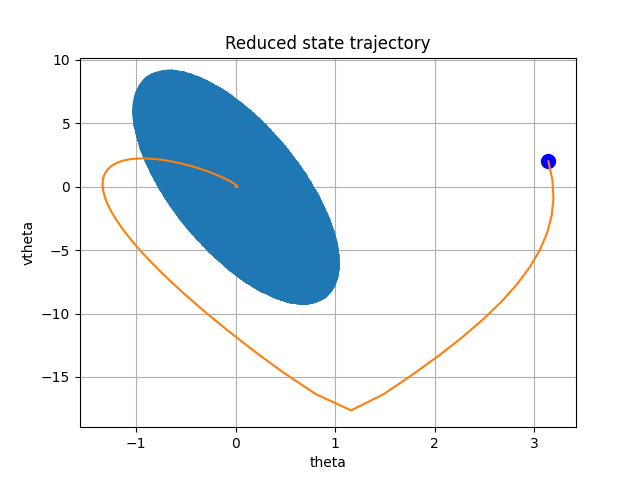
\includegraphics[width=\textwidth]{img/red_state_out}
    \end{subfigure}
    \hfill
    \begin{subfigure}{0.48\textwidth}
    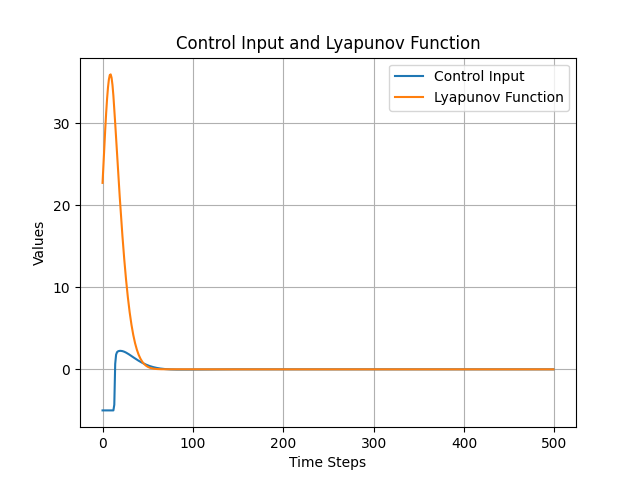
\includegraphics[width=\textwidth]{img/lyap_out}
    \end{subfigure}
    \caption{Initial state out of ROA, the system is still able to reach the origin but the Lyapunov function is not strictly decreasing}
\end{figure}

\begin{figure}[H]
    \centering
    \begin{subfigure}{0.48\textwidth}
    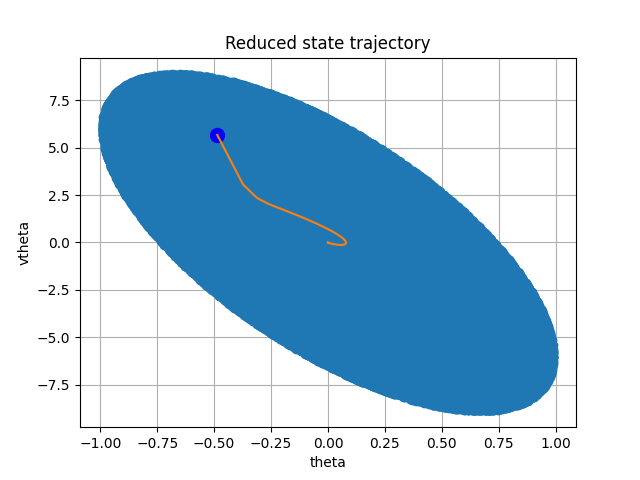
\includegraphics[width=\textwidth]{img/red_state_inside}
    \end{subfigure}
    \hfill
    \begin{subfigure}{0.48\textwidth}
    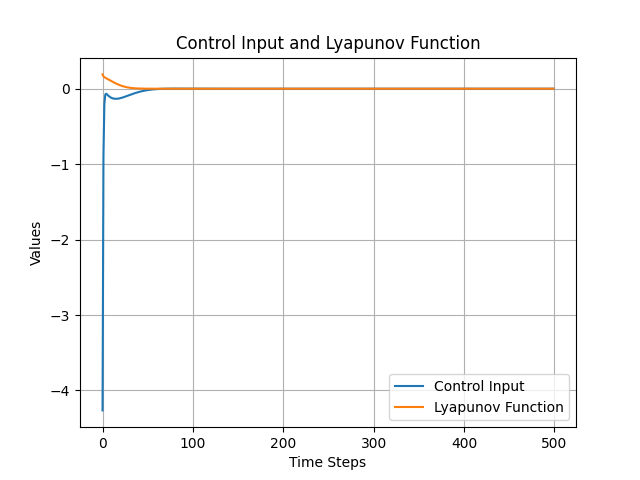
\includegraphics[width=\textwidth]{img/lyap_inside}
    \end{subfigure}
    \caption{Initial state inside the ROA, the system is able to reach the origin and the Lyapunov function is strictly decreasing}
\end{figure}

\begin{figure}[H]
    \centering
    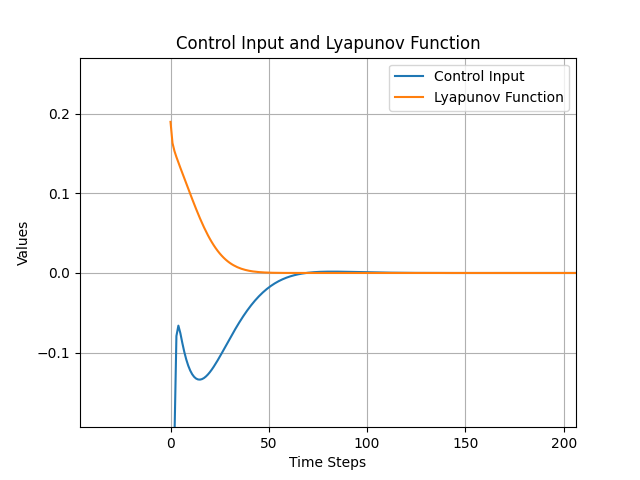
\includegraphics[width=0.5\textwidth]{img/detail_lyap}
    \caption{Detail of the Lyapunov function in the case the initial state is inside the ROA}
\end{figure}

\subsection*{Next steps}
Now the following steps regard the extraction of the "region of linearity" from this trivial 1 layer case and extend it iteratively to craft a multi-layer network controller by hand.

\pagebreak
\printbibliography


\end{document}